\chapter{Исследование существующих алгоритмов построения выпуклых оболочек} \label{chapt1}

\section{Существующие алгоритмы построения выпуклых оболочек} \label{sect1_1}

За долгое время развития вычислительной геометрии появилось огромное количество алгоритмов. Они имеют различную сложность и принцип работы. Необходимо исследовать эти алгоритмы, чтобы понимать какой алгоритм нам нужно будет сделать, чтобы с ними соперничать.

Все алгоритмы будут рассмотрены в препдположении, что все точки находятся в общем положении. Это означает, что никакие три точки не лежат на одной прямой. Это сделано только для упрощения выкладок, на практике конечно необходимо учитывать этот случай и он может быть учтён всеми представленными алгоритмами.

Также необходимо ввести предикат $ccw(A, B, C)$, который также будет использоваться для описания алгоритмов. Предикат $ccw$ показывает точки $A, B, C$ перечислены в порядке против часовой стрелки или нет. Другими словами точка $C$ должна лежать левее прямой $A, B$. На рисунке~\ref{img:ccw_1} показано, что предикат для точек $A, B, C$ выполняется, а на рисунке~\ref{img:ccw_2} он выполняться не будет.

\begin{figure}[ht]
	{\centering
		\hfill
		\subbottom[\label{img:ccw_1}]{%
			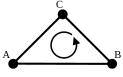
\includegraphics[width=0.4\linewidth]{ccw1}}
		\hfill
		\subbottom[\label{img:ccw_2}]{%
			\includegraphics[width=0.4\linewidth]{ccw2}}
		\hfill
	}
	\caption{Демонстрация работы предиката $ccw$}
	\label{img:ccw}
\end{figure}

Предикат $ccw$ вычисляется очень просто. Сначала необходимо посчитать детерминант $det$ матрицы \eqref{eq:det}.

\begin{equation}\label{eq:det}
det(A, B, C)= \left| \begin{array}{ccc} x_A & y_A & 1 \\ x_B & y_B & 1 \\ x_C & y_C & 1  \end{array}\right|
\end{equation}

Теперь можно определить $ccw$ через $det$ \eqref{eq:ccw}.

\begin{equation}\label{eq:ccw}
ccw(A, B, C)=det(A, B, C) > 0
\end{equation}


\subsection{Алгоритм Джарвиса} \label{subsect1_1_1}

Алгоритм Джарвиса - это один из первых придуманных алгоритмов построения выпуклой оболочки. Он был опубликован в 1972 году. %TODO ref
Этот алгоритм также называют алгоритмом заворачивания подарка, что отлично показывает суть работы алгоритма.

Пусть дано множество точек $S$. Первым делом нам надо найти такую точку $t$, чтобы было известно, что она будет лежать на выпуклой оболочке. Самый простой способ сделать это - найти левую крайнюю точку. Не теряя общности рассуждений, примем найденную точку за $t_0$. Алгоритм начинает работать при $i=0$ в точке $t_0$ и выбирает такую точку $t_{i+1}$ такую, что все остальные точки лежат правее прямой $t_i, t_{i+1}$. Также это выражается с помощью предиката \eqref{eq:ccw}:
\[
\forall p \in S \backslash \{t_i, t_{i+1}\} : ccw(t_i, t_{i+1}, p)
\]

Прямая $t_i, t_{i+1}$ на первых шагах алгоритма показана на рисунке ~\ref{img:jarvis}. Повторение этого действия пока не $t_h=p_0$ полностью построит выпуклую оболочку изначально заданного множества.

\begin{figure}[ht]
    {\centering
        \hfill
        \subbottom[\label{img:jarvis_1}]{%
            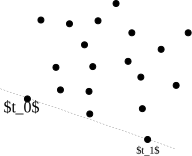
\includegraphics[width=0.4\linewidth]{jarvis1}}
        \hfill
        \subbottom[\label{img:jarvis_2}]{%
            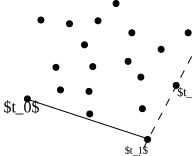
\includegraphics[width=0.4\linewidth]{jarvis2}}
        \hfill
    }
    \caption{Первые этапы работы алгоритма Джарвиса}
    \label{img:jarvis}
\end{figure}

Какова сложность алгоритма Джарвиса? Если в множестве изначально было $n$ точек, а в выпуклую оболочку попало ровно $h$ точек, то сложность алгоритма заворачивания подарка равна $O(nh)$. Доказательство этого утверждения очевидно. Так как поиск точки $t_{i+1}$ занимает проход по всему множеству точек, то это имеет сложность $O(n)$. Всего нам необходимо найти $h$ точек, так как именно столько будет находится в выпуклой оболочке.

Как видно из сложности алгоритма, он зависит не только от входных данных, но и от выходных. Это интересная особенность алгоритмов построения выпуклых оболочек, хоть и не все из них имеют сложность, зависящую от выходных данных.

\subsection{Алгоритм Грэхема} \label{subsect1_1_2}

Алгоритм Грэхема - это, наверное, самый популярный из ныне используемых алгоритмов построения выпуклых оболочек. Он очень прост в написании и при этом работает очень эффективно. Он был опубликован в 1972 году. %TODO ref

Пусть дано множество точек $S$. Первый шаг алгоритма полностью повторяет алгоритм Джарвиса - мы находим точку с самой маленькой x-координатой. Назовём эту точку $t_0$. Теперь необходимо отсортировать все остальные точки $[t_1, t_n]$ по углу относительно точки $t_0$. Это можно сделать с помощью уже знакомого предиката ccw~\eqref{eq:ccw}:
\[
A<B=ccw(t_0, A, B)
\]

Следующий этап алгоритма - это итерирование по отсортированному множеству точек. В это время все точки уже добавленные в выпуклую оболочку содержатся в стеке. Пусть сейчас добавляется точка $p$. А в стеке содержатся точки $[t_{last}, t_{last-1}, ...]$. Тогда необходимо удалить из стека такие точки, что $t_{last-1}, t_{last}, p$ образуют правый поворот. Это означает, что не выполняется $ccw(t_{last-1}, t_{last}, p)$.

На рисунке~\ref{img:graham} показан пример добавления точек при работе алгоритма Грэхема. На первом рисунке~\ref{img:graham_1} можно видеть, что добавляется точка $p_3$. Выполняется $ccw(p_1, p_2, p_3)$, поэтому точка добавляется в текущий стек. На следующем рисунке~\ref{img:graham_2} доавляется точка $p_4$, но предикат $ccw(p_2, p_3, p_4)$ не выполняется, поэтому точку $p_3$ необходимо удалить, после на рисунке~\ref{img:graham_3} видно, что это приводит к выполнению предиката $ccw(p_1, p_2, p_4)$, поэтому точка $p_4$ может быть добавлена в стек. Оставшиеся точки будут обработаны аналогичным образом, после чего мы получим готовую выпуклую оболочку состоящую из точек $p_0, p_1, p_2, p_4, p_6$.

\begin{figure}[ht]
	{\centering
		\hfill
		\subbottom[\label{img:graham_1}]{%
			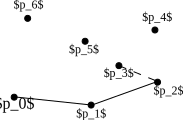
\includegraphics[width=0.3\linewidth]{graham1}}
		\hfill
		\subbottom[\label{img:graham_2}]{%
			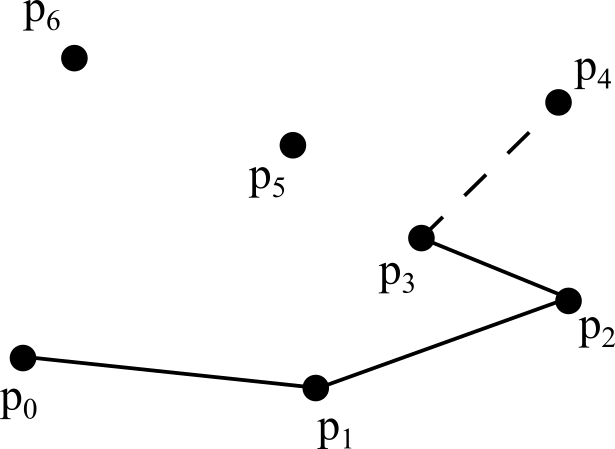
\includegraphics[width=0.3\linewidth]{graham2}}
		\hfill
		\subbottom[\label{img:graham_3}]{%
			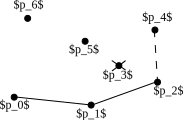
\includegraphics[width=0.3\linewidth]{graham3}}
		\hfill
	}
	\caption{Пример добавления точек при работе алгоритма Грэхема}
	\label{img:graham}
\end{figure}

Сложность этого алгоритма очень легко проанализировать. Сначала выполняется обход множества точек в поиске самой левой точки за $O(n)$. Потом необходимо отсортировать все остальные точки за $O(n \log n)$. Потом происходит обход всех точек. Заметим, что каждая точка максимум один раз добавляется в стек и один раз удаляется из него, то есть происходит $2n$ операций, что даёт сложность $O(n)$. Итоговая сложность алгоритма равна $O(n) + O(n \log n) + O(n) = O(n \log n)$.

\subsection{Разделяй и властвуй} \label{subsect1_1_3}

Принцип "Разделяй и властвуй" является очень популярным очень во многих алгоритмах в информатике. Самое знаменитое его применение - это, пожалуй, сортировка слиянием. Именно от неё во многом позаимствовал этот алгоритм для построения выпуклой оболочки множества точек.

Этот алгоритм проще всего описать с помощью рекурсивной процедуры CalcHull.

%TODO Сделать подпись не "Algorithm 1"
\begin{algorithm}
	\caption{CalcHull - функция алгоритма Разделяй и Властвуй}
	\begin{algorithmic}[1]
		\Procedure{CalcHull}{$S$}
		\If {$|S| <= 3$}
			\Return $S$
		\EndIf
		\State $leftS\gets leftOf(S)$ \Comment{Получить левую половину множества $S$}
		\State $rightS\gets rightOf(S)$ \Comment{Получить правую половину множества $S$}
		\State $leftHull\gets CalcHull(leftS)$
		\State $rightHull\gets CalcHull(rightS)$
		\State
		\Return $mergeHulls(leftHull, rightHull)$
		\EndProcedure
	\end{algorithmic}
\end{algorithm}

Сложность данного алгоритма может быть рассмотрена с помощью рекурсии, так как это и есть рекурсивная функция. Пусть изначальное множество точек состоит из $n$ элементов. Рассмотрим всё время требущееся процедуре кроме рекурсивных вызовов. Изначально нужно разделить множество точек на $leftS$ и $rightS$. Это требует $O(n)$ времени. После чего необходимо посчитать верхнюю и нижнюю касательные, и после вывести ответ. Эти действия также занимают $O(n)$ времени, что мы покажем ниже. Таким образом время может быть описано рекурсивной формулой~\ref{eq:mergeHullAnalysisBegin}.
\begin{equation}\label{eq:mergeHullAnalysisBegin}
T(n) = 3n + 2T(n/2)
\end{equation}

Как видно из ~\ref{eq:mergeHullAnalysisEnd}, сложность работы алгоритма Разделяй и Властвуй равна $O(n \log n)$.

\[
T(n) = cn \log n
\]
\[
T(n) = 3n + cn \log n/2 = 3n - cn \log 2 + cn \log n = (3 - c \log 2)n + cn \log n
\]
\begin{equation}\label{eq:mergeHullAnalysisEnd}
T(n) = 3/(\log 2)n \log n = O(n \log n)
\end{equation}

Единственное, что осталось доказать - это что можно вычислить верхнюю и нижнюю касательные за $O(n)$ время. Мы будем рассматривать только как считать нижнюю касательную, потому что верхняя может быть рассмотрена симметрично. Итак, пусть $a$ - это самая правая точка $leftHull$, а $b$ - это самая левая точка $rightHull$. Тогда пока $ab$ это не нижняя касательная ни для $leftHull$, ни для $rightHull$, необходимо попытаться продвинуть точку $a$ максимально вниз пока $ab$ не будет являтся нижней касательной для $leftHull$, а потом продвинуть точку $b$ пока $ab$ не будет являтся нижней касательной для $rightHull$. Этот процесс показан на рисунке~\ref{img:merge_1}. Финальный результат показан на втором рисунке~\ref{img:merge_2}.

\begin{figure}[ht]
	{\centering
		\hfill
		\subbottom[\label{img:merge_1}]{%
			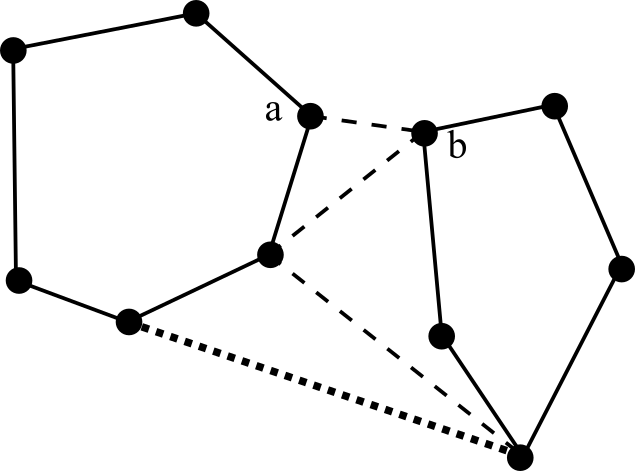
\includegraphics[width=0.4\linewidth]{merge1}}
		\hfill
		\subbottom[\label{img:merge_2}]{%
			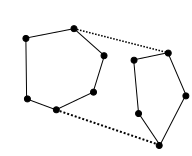
\includegraphics[width=0.4\linewidth]{merge2}}
		\hfill
	}
	\caption{Нахождение верхней и нижней касательных}
	\label{img:merge}
\end{figure}


Проверять является ли прямая нижней касательной к выпуклой оболочке очень просто. Достаточно проверить лежат ли соседние к $a, b$ точки выше этой прямой.

Очевидно, что алгоритм нахождения нижней касательной работает за $O(n)$, поэтому анализ сложности, показанный выше, верен.

\subsection{Quickhull} \label{subsect1_1_4}

Логическим продолжением алгоритма, который основан на сортировке слиянием является алгоритм основанный на быстрой сортировке. Это довольно простой и в то же время быстро работающий алгоритм. В точности как и быстрая сортировка, данный алгоритм имеет сложность $O(n \log n)$. Но в худшем случае он может работать за $O(n^2)$. Что отличет алгоритм нахождения выпуклой оболочки множества точек Quickhull и алгоритм сортировки Quicksort - это невозможность случайной перестановки до работы алгоритма, чтобы алгоритм всегда работал с сложностью $O(n \log n)$.

Самая главная идея, которая лежит в основе данного алгоритма - это убирание ненужных точек, чем раньше мы их отбросим, тем лучше. Таких точек очень много внутри выпуклой оболочки. Как правило большинство точек изначального множества окажется внутри.

Первый шаг алгоритма - это найти четыре точки у которых будут минимальные/максимальные x/y-координаты. Это даёт нам изначальное приближение к выпуклой оболочке, которую мы построим в итоге. Очевидно, что точки, который будут лежать внутри получившегося четырёхугольника можно не рассматривать, так как они будут точно лежать внутри выпуклой оболочки. Это показано на рисунке %TODO: добавить рисунок

\subsection{Инкрементальный алгоритм} \label{subsect1_1_5}

\subsection{Алгоритм Чана} \label{subsect1_1_6}

\section{Анализ текущего состояния алгоритмов и выявление проблемы} \label{sect1_2}

\section{Требования, предъявляемые к разрабатываемому алгоритму} \label{sect1_3}







